\documentclass{article}\usepackage[]{graphicx}\usepackage[]{color}
% maxwidth is the original width if it is less than linewidth
% otherwise use linewidth (to make sure the graphics do not exceed the margin)
\makeatletter
\def\maxwidth{ %
  \ifdim\Gin@nat@width>\linewidth
    \linewidth
  \else
    \Gin@nat@width
  \fi
}
\makeatother

\definecolor{fgcolor}{rgb}{0.345, 0.345, 0.345}
\newcommand{\hlnum}[1]{\textcolor[rgb]{0.686,0.059,0.569}{#1}}%
\newcommand{\hlstr}[1]{\textcolor[rgb]{0.192,0.494,0.8}{#1}}%
\newcommand{\hlcom}[1]{\textcolor[rgb]{0.678,0.584,0.686}{\textit{#1}}}%
\newcommand{\hlopt}[1]{\textcolor[rgb]{0,0,0}{#1}}%
\newcommand{\hlstd}[1]{\textcolor[rgb]{0.345,0.345,0.345}{#1}}%
\newcommand{\hlkwa}[1]{\textcolor[rgb]{0.161,0.373,0.58}{\textbf{#1}}}%
\newcommand{\hlkwb}[1]{\textcolor[rgb]{0.69,0.353,0.396}{#1}}%
\newcommand{\hlkwc}[1]{\textcolor[rgb]{0.333,0.667,0.333}{#1}}%
\newcommand{\hlkwd}[1]{\textcolor[rgb]{0.737,0.353,0.396}{\textbf{#1}}}%
\let\hlipl\hlkwb

\usepackage{framed}
\makeatletter
\newenvironment{kframe}{%
 \def\at@end@of@kframe{}%
 \ifinner\ifhmode%
  \def\at@end@of@kframe{\end{minipage}}%
  \begin{minipage}{\columnwidth}%
 \fi\fi%
 \def\FrameCommand##1{\hskip\@totalleftmargin \hskip-\fboxsep
 \colorbox{shadecolor}{##1}\hskip-\fboxsep
     % There is no \\@totalrightmargin, so:
     \hskip-\linewidth \hskip-\@totalleftmargin \hskip\columnwidth}%
 \MakeFramed {\advance\hsize-\width
   \@totalleftmargin\z@ \linewidth\hsize
   \@setminipage}}%
 {\par\unskip\endMakeFramed%
 \at@end@of@kframe}
\makeatother

\definecolor{shadecolor}{rgb}{.97, .97, .97}
\definecolor{messagecolor}{rgb}{0, 0, 0}
\definecolor{warningcolor}{rgb}{1, 0, 1}
\definecolor{errorcolor}{rgb}{1, 0, 0}
\newenvironment{knitrout}{}{} % an empty environment to be redefined in TeX

\usepackage{alltt}
\usepackage{color}
\usepackage[T1]{fontenc}

%% packages
\usepackage{scrtime}  % for \thistime (this package MUST be listed first!)
\usepackage[margin=1in]{geometry} % page layout
\usepackage{amsmath}  % essential for cases environment
\usepackage{amsthm}   % for theorems and proofs
\usepackage{amsfonts} % mathbb
\usepackage{graphics,graphicx}
\usepackage{multirow} % fancy tables
\usepackage{wasysym}  % circle symbols (including half-filled circles)
\usepackage{enumerate}% fancier enumeration (e.g., a,b,c, ...)
%\usepackage{xcolor}
\usepackage{color}

\usepackage{amssymb,latexsym,setspace}
%%\usepackage[colorlinks,linkcolor=blue]{hyperref}
%\usepackage[colorlinks=true,allcolors=blue]{hyperref}
\usepackage{xspace}
\usepackage{subfigure}
\usepackage{lineno}
\usepackage{fancyhdr}
\usepackage[english]{babel}  %% for texi2dvi ~ bug
\usepackage[normalem]{ulem}
\usepackage{tikz} % http://www.texample.net/tikz/examples/tikzdevice-demo/
  % N.B. version 0.6.3 of tikzDevice from Rforge is required!!
%% improve figure caption typsetting:  (see ~/tex/caption.pdf for manual)
\usepackage[footnotesize,bf]{caption}
\usepackage{placeins} % \FloatBarrier

%% comments
\newcommand{\de}[1]{{\color{red}{\bfseries DE:} #1}}

%% for solutions to multiple choice questions:
\newcommand{\correct}{{\color{blue}\fbox{\color{red}\checkmark} }}

%% macros
\newcommand{\reals}{\mathbb{R}}
\newcommand{\term}[1]{{\bfseries\slshape #1}}
\newcommand{\Ker}{{\text{Ker}\,}}
\newcommand{\Range}{{\text{Range}\,}}
\newcommand{\diag}{{\text{diag}}}
\newcommand{\alg}{{\text{alg}}}
\newcommand{\geom}{{\text{geom}}}
\newcommand{\norm}[1]{\left\|#1\right\|}
\newcommand{\abs}[1]{\left|#1\right|}
\newcommand{\R}{{\cal R}}
\newcommand{\eps}{\varepsilon}
\newcommand{\B}{\cal B}
\newcommand{\Tinf}{T_\textrm{inf}}
\newcommand{\Shat}{{\hat{S}}}
\newcommand{\Ihat}{{\hat{I}}}
\newcommand{\ie}{\emph{i.e., }}
\newcommand{\eg}{\emph{e.g., }}
\newcommand{\Rlogo}{\protect
\includegraphics[height=2ex,keepaspectratio]{images/Rlogo.pdf}\xspace}
\newcommand{\XPPAUT}{\texttt{XPPAUT}\xspace}
\newcommand{\etal}{\textit{et al}.\xspace}
\newcommand\emphblue[1]{\emph{\color{blue}#1}}

% citation macros
\newcommand{\citen}[1]{\cite{#1}}

% other macros
\newcommand{\avg}[1]{{\left\langle#1\right\rangle}}
\newcommand{\var}[1]{\textrm{var}\left(#1\right)}
\newcommand{\sem}[1]{\textrm{sem}\left(#1\right)}
\newcommand{\natinf}{{\mathcal I}}
\newcommand{\find}{f_{\textrm{i}}}
\newcommand{\fpop}{f_{\textrm{p}}}
\newcommand{\logit}{\textrm{logit}}
\newcommand{\sign}{\textrm{sign}}
\newcommand{\logistic}{\textrm{logistic}}
\newcommand{\code}[1]{{\tt #1}}
\newcommand{\magcode}[1]{{\tt\color{magenta}#1}}
\newcommand{\redcode}[1]{{\tt\color{red}#1}}
\newcommand{\blackcode}[1]{{\tt\color{black}#1}}

%%%%%%%%%%%%%%%%%%%
%% JOURNAL NAMES %%
%%%%%%%%%%%%%%%%%%%
\def\AJE{{\it American Journal of Epidemiology\/}}
\def\PNAS{PNAS}
\def\JAMA{JAMA}
\def\BMB{{\it Bulletin of Mathematical Biology\/}}

% references
\newcommand{\eref}[1]{Equation~\eqref{E:#1}}
\newcommand{\fref}[1]{Figure~\ref{F:#1}}
\newcommand{\tref}[1]{Table~\ref{T:#1}}
\newcommand{\sref}[1]{\S\ref{S:#1}}
% other macros
\newcommand{{\Reff}}{{\mathcal{R}}_{\rm eff}}
\newcommand{{\Sinit}}{S_{\rm init}}
\newcommand{\supp}{Supplementary Information}
\newcommand{\StoppedHere}{\bigskip\bigskip{\textcolor{red}{\hrule\centerline{\bfseries STOPPED HERE}\hrule}}\bigskip\bigskip}
\newcommand{\colvec}[2]{\begin{pmatrix}#1\\#2\end{pmatrix}}
\newcommand{\diagmat}[3]{\begin{pmatrix}#1&0&0\\0&#2&0\\0&0&#3\end{pmatrix}}

\newcommand{\solution}[1]{{\hfill\break\vspace{-0.5\baselineskip}\break\color{blue}\emph{Solution: }#1}}
\newcommand{\tr}{\text{tr}}

\newcommand{\thickredline}{\bigskip{\color{red}\hrule height 5pt}\bigskip}

%% for assignment 3:
\newtheorem{theorem}{Theorem}
\newtheorem{remark}{Remark}
\newcommand{\openset}{{\mathcal O}}
%\newcommand{\C}{{\mathcal C}}

%% underline with smash through:
\newcommand*{\undersmash}[1]{\underline{\smash{#1}}}

%% referring to TeX macros
\newcommand\ttbackslash{{\tt\char`\\}}
\newcommand{\macro}[1]{{\tt\ttbackslash#1}}

%%%%%%%%%%%%%%%%%%%%%%%%%%%%%%%%%%%%%
%%http://tex.stackexchange.com/questions/128424/how-to-create-email-hyperlink-with-predefined-subject-in-latex
\usepackage{etoolbox}
\makeatletter
\newcommand\myemail[3]{%                %\newcommand\tpj@compose@mailto[3]{%
\edef\@tempa{mailto:#1?subject=#2 }%
\edef\@tempb{\expandafter\html@spaces\@tempa\@empty}%
\href{\@tempb}{#3}}

\catcode\%=11
\def\html@spaces#1 #2{#1%20\ifx#2\@empty\else\expandafter\html@spaces\fi#2}
\catcode\%=14
\makeatother
%%%%%%%%%%%%%%%%%%%%%%%%%%%%%%%%%%%%%
\newcommand{\thiscoursecode}{4MB3}
\newcommand{\myemaillink}{\myemail{earn@math.mcmaster.ca}{Math \thiscoursecode: }{earn@math.mcmaster.ca}}

\IfFileExists{upquote.sty}{\usepackage{upquote}}{}
\begin{document}

\title{Mathematics 747 Assignment 2}
\author{Zachary Levine}
\date{\today}
\maketitle

The following assignment was completed using the \texttt{McMasterPandemic} $\Rlogo$ package.

\section{McMasterPandemic shiny Improvements}
I implemented the following bug fixes for the Shiny:
\begin{itemize}
\item Fixed a bug (at Luka and Vlad's sugegstion) where setting the population size (and several other parameters) explicitly by typing into the box would force the slider and the text input box out of sync.
\item Fixed a bug (at Aigerim's suggestion) where time varying transmission rates could not be implimented after noise had been added to the graph.
\end{itemize}

Parts two and three were already complete.

\section{Part four: Simulating an epidemic}
 I spent many hours trying to find parameter settings to make the first wave of COVID-19 in Ontario. I first spent a very long time trying to do so without implementing time-varying transmission rates, and could not come up with a simulation that was even remotely close to the first wave of reported cases in Ontario. Eventually, I had to implement two time-varying changes for \texttt{beta0}, the baseline transmission rate across categories. I tried to find a match between the \texttt{report} column of the simulation and daily reported case counts of COVID-19 in Ontario. Below, please find my result.
 
\begin{knitrout}
\definecolor{shadecolor}{rgb}{0.969, 0.969, 0.969}\color{fgcolor}
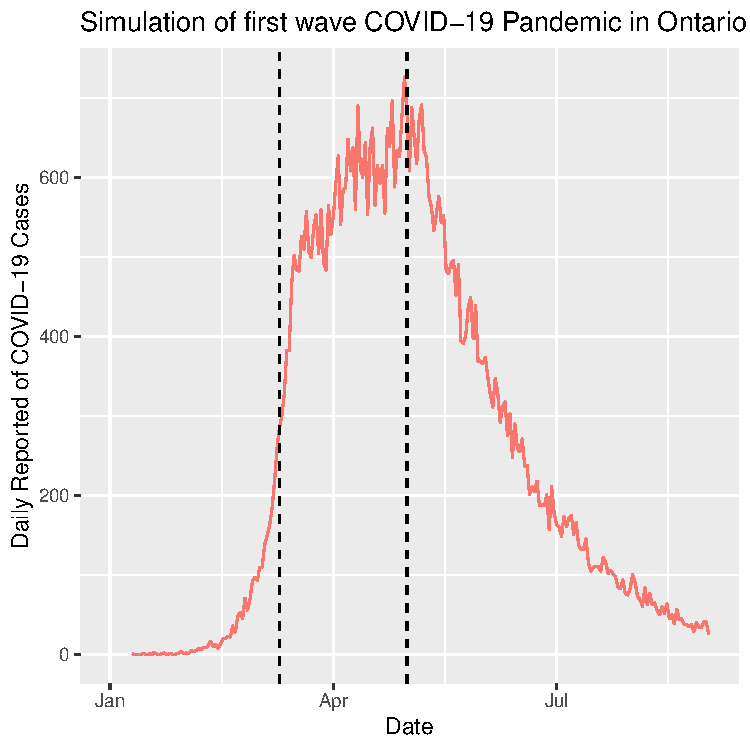
\includegraphics[width=\maxwidth]{figure/init-1} 

\end{knitrout}


\section{Part five: parameter fitting}
Now, assuming that my simulation of the first wave in Ontario is correct, we will use the fitting machinery in \texttt{McMasterPandemic}, namely the method \texttt{calibrate} to estimate the model parameter for \texttt{beta0} that we started with. Then, we will plot the result.

\begin{knitrout}
\definecolor{shadecolor}{rgb}{0.969, 0.969, 0.969}\color{fgcolor}
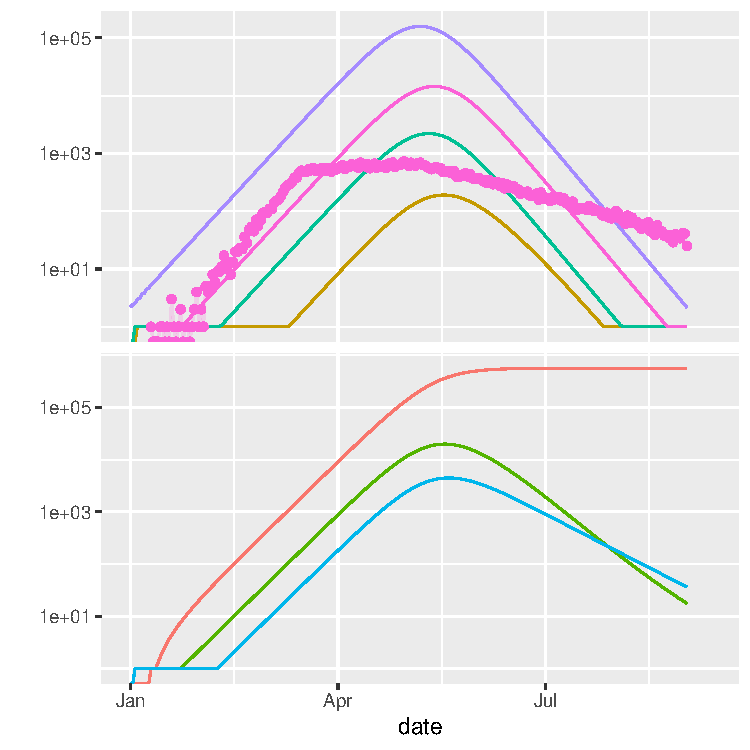
\includegraphics[width=\maxwidth]{figure/main-1} 

\end{knitrout}

Visual inspection of the plot confirms that we have a decent model fit. If we compare the estimated parameters with the known ones that we used to generate the simulation, we see a somewhat reasonable match as well.

\begin{knitrout}
\definecolor{shadecolor}{rgb}{0.969, 0.969, 0.969}\color{fgcolor}
\begin{tabular}{r|r|r}
\hline
beta0 initial values & beta0 first time change & beta0 second time change\\
\hline
0.929400 & 0.7671000 & 0.7261000\\
\hline
0.892804 & 0.6256154 & 0.8225528\\
\hline
\end{tabular}

\begin{kframe}\begin{verbatim}
## $params
## $params$beta0
## [1] 0.892804
## 
## 
## $rel_beta0
## [1] 0.6256154 0.8225528
\end{verbatim}
\end{kframe}
\end{knitrout}

We hypothesize that including both process error and observation error does worsened our parameter estimates significantly. However, we conclude our section with some feedback on the \texttt{McMasterPandemic} package.

\section{Part six: Feedback on \texttt{McMasterPandemic}}
Overall, I really enjoyed working with the \texttt{McMasterPandemic} package.

\end{document}
